\documentclass[11pt]{article}

\usepackage[margin=1in]{geometry} 
\usepackage{amsmath,amsthm,amssymb, graphicx, multicol, array}
\usepackage{hyperref}

\newcommand{\N}{\mathbb{N}}
\newcommand{\Z}{\mathbb{Z}}
 
\newenvironment{problem}[2][Problem]{\begin{trivlist}
\item[\hskip \labelsep {\bfseries #1}\hskip \labelsep {\bfseries #2.}]}{\end{trivlist}}

\begin{document}
CSCI181AF: Advanced Data Structures\\
09/07/2022
\begin{center}
    \bf{Writeup HW \#1}
\end{center}
\subsection{Introduction}
In this writeup, we will be evaluating two different algorithms written in two different programming languages ability to approximate $\pi$. The first Python algorithm calculates $\pi$ by simulating the inscribing of a circle in a square by selecting random points in the square and checking if they are in said circle giving us $\approx \frac{\pi}{4}$. In comparison, the C++ algorithm uses the average value of the function $f(x) = \sqrt{1-x^2}$ on the interval $[0,1]$ to approximate $\frac{\pi}{4}$. Both algorithms used $n$ points.
\subsection{Python Approximation}
From the Python approximation, we were able to generate the following approximations of $\pi$ for $n = 10000, 1000000, 25000000$ points.
\begin{center}
    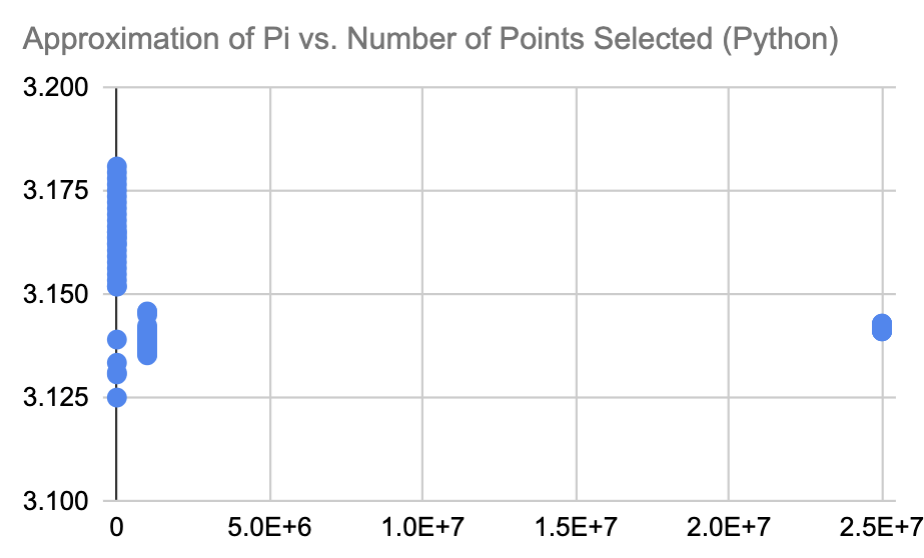
\includegraphics[scale = 0.4]{hw1image1.png} 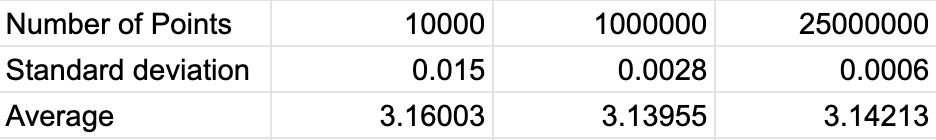
\includegraphics[scale = 0.4]{hw1image3.png}
\end{center}
\subsection{C++ Approximation}
From the C++ approximation, we were able to generate the following approximations of $\pi$ for $n = 10000, 1000000, 25000000$ points.
\begin{center}
    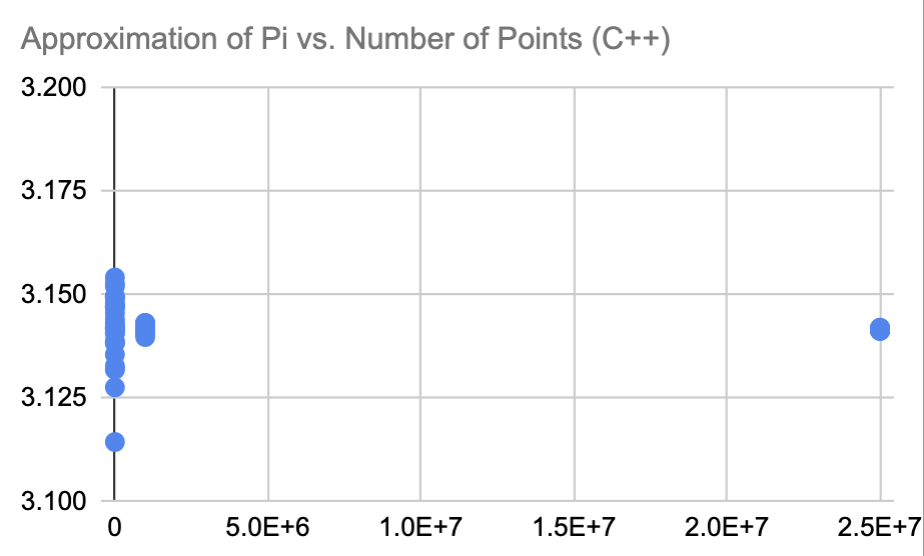
\includegraphics[scale = 0.4]{hw1image2.png} 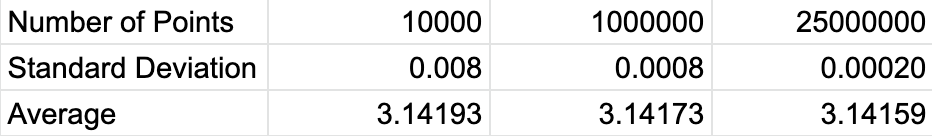
\includegraphics[scale = 0.4]{hw1image4.png}
\end{center}
\subsection{Conclusion}
One thing to note when comparing the two algorithms, is that the C++ algorithm was able to approximate $\pi$ more quickly (timewise) and with a higher degree of accuracy for a lower value of $n$, as indicated by the lesser standard deviation for $n = 10000$ and an average that is closer to $\pi$. Similarly, for larger values of $n$, the C++ algorithm was able to obtain an average value closer to $\pi$, with a lesser spread as seen by the case where $n = 25000000$ where the standard deviation of C++ Approx $<$ standard deviation of Python Approx,
all while $|\pi - approx|$ was minimized under the C++ algorithm for each of our $n$ point experiments.
\end{document}